\subsection{Vision-based docking and fiducial markers}

Passive visual markers are high-contrast patterns (typically black and white pixelated squared markers) detected by a camera and used for pose estimation. Early work from Maire's Starbug dock system designed custom geometries which used a binary encoded pole as a passive black and white target mounted inside a suspended docking station. The pattern is designed so that it is visible from any arbitrary yaw, roll or pitch angle and also serves as a structural station that the AUV can grip on. Detection is performed with a fast Haar feature template matcher over the image, where the 'dash-dot-dash' black and white pattern is scored over multiple scales, positions and image rotations to locate the camera pose relative to the dock \cite{maire2009vision}. As the AUV approaches closer, the system switches to shorter templates to maintain more precise tracking at close distance. This method purely using a high contrast pattern can deliver robust homing without any powered beacons, however, it is limited by the CPU cost of the template search over multiple scales and rotations, and restricts design flexibility for the dock station. Later work on general visual application for regular (standardised) fiducial systems like AprilTag and ArUco follows the standard method of obtaining pose of the markers from camera frame, which square markers are detected by adaptive thresholding and decoded against a dictionary, with the four corners feeding a Perspective-n-Point (PnP) solution for full 6-DOF pose \cite{garrido2014automatic, kalaitzakis2021fiducial}. Notably, Xu's AUV navigation system detects a grid of multiple markers for improved accuracy \cite{xu2021underwater}. The ArUco library first decodes each marker ID and recovers the marker's pose relative to the camera. Then, Xu's custom noise model computes an optimal combined pose estimate from all visible markers, improving accuracy and robustness against individual detection errors. Vision positioning with two cameras has likewise been used in AUV docking experiments \cite{li2015auv}. The same principle applies to Romero-Ram\'irez's fractal markers, which survive across the long to short range span by having ``an aggregation of squared markers, one into another, in a recursive manner'', see Figure~\ref{fig:fractal-marker} \cite{romeroramirez2019fractal}.

\begin{figure}[H]
    \centering
    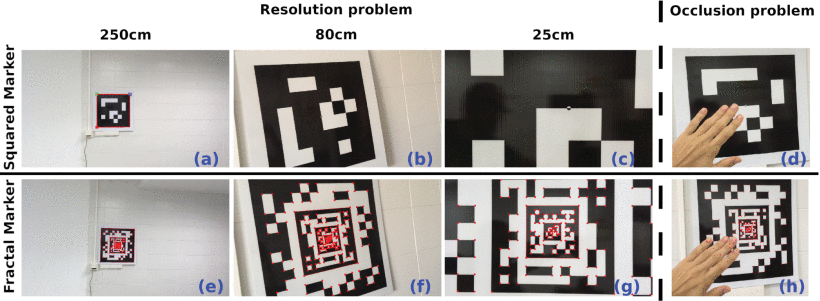
\includegraphics[width=0.6\textwidth]{Figures/fractal_markers_new_approach.png}
    \caption{Result of the Fractal Markers against regular squared markers at different distances and occlusion, where Fractal Markers can be detected in more cases than regular squared markers \cite{romeroramirez2019fractal}.}
    \label{fig:fractal-marker}
\end{figure}

\noindent There is little design guidance on how these marker sets should be arranged. Wang's controlled study on marker size, count and distribution found that apparent size is the dominant factor for localisation accuracy, while marker count and placement only have secondary effects \cite{wang2023effect}. The dock layout of this work assumes the same ordering. The closest deployed system to this work is G\"unzel's resident mini-ROV, which docks onto a multi-size ArUco layout at 90~m depth, fused through an extended Kalman filter, and reports a 90\% docking success rate \cite{gunzel2026docking}. This architecture matches the size-graded layout and filter design of this work. However, the dock station is static, and the marker sizes were selected through simulator experiments without water optics, so the underwater perception envelope remains unmeasured. For underwater detection performance, dos Santos Cesar et al. evaluated three fiducial systems (ArUco, AprilTag and ARToolKit) in tank conditions, measuring the smallest detectable size, maximum viewing angle and detection range across six turbidity levels \cite{cesar2015evaluation}. This study establishes apparent size and turbidity as the two main variables of underwater fiducial detection. Among the three libraries, ArUco showed the highest sensitivity to turbidity, with its required marker size growing at the fastest rate.

Most recently, Ni et al. proposed a hybrid active and passive docking marker where a printed AprilTag is placed at the center of the dock station, surrounded by an array of five LED lights \cite{ni2025vision}, following Trslic's four light beacon active marker design \cite{trslic2020vision}. A custom YOLO-D model is trained to simultaneously detect the LED array and the AprilTag in raw underwater images.
\begin{figure}[H]
    \centering
    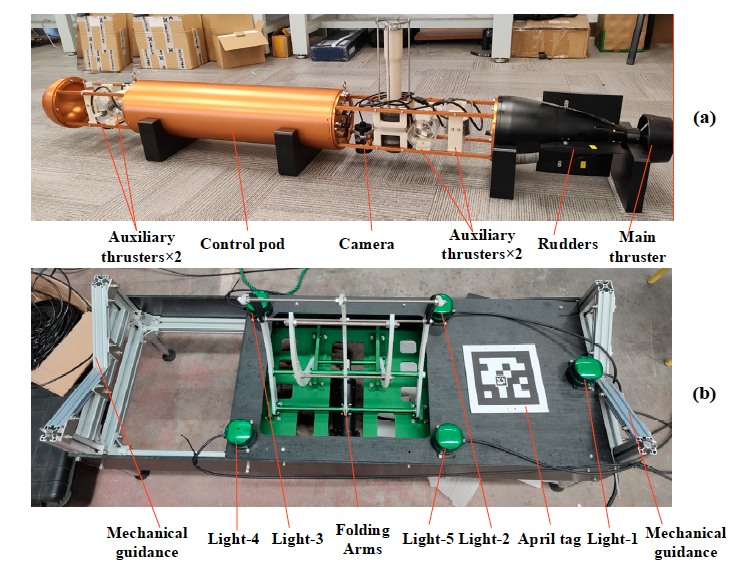
\includegraphics[width=0.6\textwidth]{Figures/msae-dock-and-auv-diagram.png}

    \caption{Example of an underwater docking station and vehicle: (a) AUV; (b) Docking station with five green LED beacons (Light-1 to Light-5), AprilTag marker at the center and v-shaped mechanical guides.\cite{ni2025vision}}
    \label{fig:ni-dock}
\end{figure}
\noindent Ni et al.'s AUV docking guidance is composed of two levels of detection:
\begin{itemize}
    \item Level I: the LED array is used as visual markers for pose estimation. However, at close range, the light scattering can introduce errors in estimating the center of the guidance light source.
    \item Level II: the AprilTag is used for precise pose estimation. However, this guidance method is limited by the detection range and visibility of the tag under turbidity, water quality and illumination.
\end{itemize}
The docking process begins by capturing an image, which is preprocessed through configured filters to minimise noise in the image. The YOLO-D model then detects the center \(X_L\) of the LED array and the AprilTag region of interest (ROI) in the image frame. In Level I guidance, the obtained \(X_L\) is used to compute a coarse position \(P_L\) of the docking station relative to the AUV. In Level II guidance, the AprilTag corners \(X_A\) are extracted from the ROI and used to compute a precise pose \(P_A\) via PnP. Finally, the pose estimates from both levels are fused to compute the overall \(P_{out}\), following the formula

\[ P_{out} = K_1 P_L + K_2 P_A \]

where \(K_1\) and \(K_2\) are weight matrices adjusted according to the conditions, shifting toward the surviving channel when poor water quality prevents one marker type from being detected. This fusion allows the system to leverage the long-range detection of the LED array while maintaining the precision of the AprilTag when visible.

Learning-based detection is the other active research direction. Standard object detectors are typically trained on terrestrial images, so their performance degrades in low-light and low-contrast conditions \cite{DAS20253042}, which are the typical conditions of underwater scenes, and motivated a few underwater-specific variants. For example, Pan's YOLOv9s-UI adds attention modules for underwater object detection \cite{app14167162}, and Ni's YOLO-D (described above) augments a YOLO backbone with multi-scale feature fusion and adaptive kernels to detect distant lights and partially visible tags \cite{ni2025vision}. Another, Sans-Muntadas trained a CNN that regresses the heading error to the dock directly from raw images, replacing explicit marker detection entirely \cite{sans2019learning}. However, this method degrades at close range where visible features vanish. In practice, these learning methods serve as the detection front end of a larger system, while the metric pose is still recovered geometrically from the marker corners. They also carry extra costs in training data, onboard compute and validation effort, which are significant for small / low-cost ROV platforms. For this reason, this thesis stays with the classical fiducial pipeline. The detection algorithm is mature and cheap, and the open question is the operating envelope of the detector rather than the detector itself.
